%
% This is an example LaTeX file which uses the SANDreport class file.
% It shows how a SAND report should be formatted, what sections and
% elements it should contain, and how to use the SANDreport class.
% It uses the LaTeX article class, but not the strict option.
% ItINLreport uses .eps logos and files to show how pdflatex can be used
%
% Get the latest version of the class file and more at
%    http://www.cs.sandia.gov/~rolf/SANDreport
%
% This file and the SANDreport.cls file are based on information
% contained in "Guide to Preparing {SAND} Reports", Sand98-0730, edited
% by Tamara K. Locke, and the newer "Guide to Preparing SAND Reports and
% Other Communication Products", SAND2002-2068P.
% Please send corrections and suggestions for improvements to
% Rolf Riesen, Org. 9223, MS 1110, rolf@cs.sandia.gov
%
\documentclass[pdf,12pt]{INLreport}
% pslatex is really old (1994).  It attempts to merge the times and mathptm packages.
% My opinion is that it produces a really bad looking math font.  So why are we using it?
% If you just want to change the text font, you should just \usepackage{times}.
% \usepackage{pslatex}
\usepackage{times}
\usepackage[FIGBOTCAP,normal,bf,tight]{subfigure}
\usepackage{amsmath}
\usepackage{amssymb}
\usepackage{bigints}
\usepackage{pifont}
\usepackage{enumerate}
\usepackage{listings}
\usepackage{fullpage}
\usepackage{xcolor}          % Using xcolor for more robust color specification
\usepackage{ifthen}          % For simple checking in newcommand blocks
\usepackage{textcomp}
\usepackage{mathtools} 
\usepackage[toc,page]{appendix}
%\usepackage[table,xcdraw]{xcolor}
%\usepackage{authblk}         % For making the author list look prettier
%\renewcommand\Authsep{,~\,}

% Custom colors
\definecolor{deepblue}{rgb}{0,0,0.5}
\definecolor{deepred}{rgb}{0.6,0,0}
\definecolor{deepgreen}{rgb}{0,0.5,0}
\definecolor{forestgreen}{RGB}{34,139,34}
\definecolor{orangered}{RGB}{239,134,64}
\definecolor{darkblue}{rgb}{0.0,0.0,0.6}
\definecolor{gray}{rgb}{0.4,0.4,0.4}

\lstset {
  basicstyle=\ttfamily,
  frame=single
}

\setcounter{secnumdepth}{5}
\lstdefinestyle{XML} {
    language=XML,
    extendedchars=true,
    breaklines=true,
    breakatwhitespace=true,
%    emph={name,dim,interactive,overwrite},
    emphstyle=\color{red},
    basicstyle=\ttfamily,
%    columns=fullflexible,
    commentstyle=\color{gray}\upshape,
    morestring=[b]",
    morecomment=[s]{<?}{?>},
    morecomment=[s][\color{forestgreen}]{<!--}{-->},
    keywordstyle=\color{cyan},
    stringstyle=\ttfamily\color{black},
    tagstyle=\color{darkblue}\bf\ttfamily,
    morekeywords={name,type},
%    morekeywords={name,attribute,source,variables,version,type,release,x,z,y,xlabel,ylabel,how,text,param1,param2,color,label},
}
\lstset{language=python,upquote=true}

\usepackage{titlesec}
\newcommand{\sectionbreak}{\clearpage}
\setcounter{secnumdepth}{4}

%\titleformat{\paragraph}
%{\normalfont\normalsize\bfseries}{\theparagraph}{1em}{}
%\titlespacing*{\paragraph}
%{0pt}{3.25ex plus 1ex minus .2ex}{1.5ex plus .2ex}

%%%%%%%% Begin comands definition to input python code into document
\usepackage[utf8]{inputenc}

% Default fixed font does not support bold face
\DeclareFixedFont{\ttb}{T1}{txtt}{bx}{n}{9} % for bold
\DeclareFixedFont{\ttm}{T1}{txtt}{m}{n}{9}  % for normal

\usepackage{listings}

% Python style for highlighting
\newcommand\pythonstyle{\lstset{
language=Python,
basicstyle=\ttm,
otherkeywords={self, none, return},             % Add keywords here
keywordstyle=\ttb\color{deepblue},
emph={MyClass,__init__},          % Custom highlighting
emphstyle=\ttb\color{deepred},    % Custom highlighting style
stringstyle=\color{deepgreen},
frame=tb,                         % Any extra options here
showstringspaces=false            %
}}


% Python environment
\lstnewenvironment{python}[1][]
{
\pythonstyle
\lstset{#1}
}
{}

% Python for external files
\newcommand\pythonexternal[2][]{{
\pythonstyle
\lstinputlisting[#1]{#2}}}

\lstnewenvironment{xml}
{}
{}

% Python for inline
\newcommand\pythoninline[1]{{\pythonstyle\lstinline!#1!}}

% Named Colors for the comments below (Attempted to match git symbol colors)
\definecolor{RScolor}{HTML}{8EB361}  % Sonat (adjusted for clarity)
\definecolor{DPMcolor}{HTML}{E28B8D} % Dan
\definecolor{JCcolor}{HTML}{82A8D9}  % Josh (adjusted for clarity)
\definecolor{AAcolor}{HTML}{8D7F44}  % Andrea
\definecolor{CRcolor}{HTML}{AC39CE}  % Cristian
\definecolor{RKcolor}{HTML}{3ECC8D}  % Bob (adjusted for clarity)
\definecolor{DMcolor}{HTML}{276605}  % Diego (adjusted for clarity)
\definecolor{PTcolor}{HTML}{990000}  % Paul

\def\DRAFT{} % Uncomment this if you want to see the notes people have been adding
% Comment command for developers (Should only be used under active development)
\ifdefined\DRAFT
  \newcommand{\nameLabeler}[3]{\textcolor{#2}{[[#1: #3]]}}
\else
  \newcommand{\nameLabeler}[3]{}
\fi
\newcommand{\alfoa}[1] {\nameLabeler{Andrea}{AAcolor}{#1}}
\newcommand{\cristr}[1] {\nameLabeler{Cristian}{CRcolor}{#1}}
\newcommand{\mandd}[1] {\nameLabeler{Diego}{DMcolor}{#1}}
\newcommand{\maljdan}[1] {\nameLabeler{Dan}{DPMcolor}{#1}}
\newcommand{\cogljj}[1] {\nameLabeler{Josh}{JCcolor}{#1}}
\newcommand{\bobk}[1] {\nameLabeler{Bob}{RKcolor}{#1}}
\newcommand{\senrs}[1] {\nameLabeler{Sonat}{RScolor}{#1}}
\newcommand{\talbpaul}[1] {\nameLabeler{Paul}{PTcolor}{#1}}
% Commands for making the LaTeX a bit more uniform and cleaner
\newcommand{\TODO}[1]    {\textcolor{red}{\textit{(#1)}}}
\newcommand{\xmlAttrRequired}[1] {\textcolor{red}{\textbf{\texttt{#1}}}}
\newcommand{\xmlAttr}[1] {\textcolor{cyan}{\textbf{\texttt{#1}}}}
\newcommand{\xmlNodeRequired}[1] {\textcolor{deepblue}{\textbf{\texttt{<#1>}}}}
\newcommand{\xmlNode}[1] {\textcolor{darkblue}{\textbf{\texttt{<#1>}}}}
\newcommand{\xmlString}[1] {\textcolor{black}{\textbf{\texttt{'#1'}}}}
\newcommand{\xmlDesc}[1] {\textbf{\textit{#1}}} % Maybe a misnomer, but I am
                                                % using this to detail the data
                                                % type and necessity of an XML
                                                % node or attribute,
                                                % xmlDesc = XML description
\newcommand{\default}[1]{~\\*\textit{Default: #1}}
\newcommand{\nb} {\textcolor{deepgreen}{\textbf{~Note:}}~}


%%%%%%%% End comands definition to input python code into document

%\usepackage[dvips,light,first,bottomafter]{draftcopy}
%\draftcopyName{Sample, contains no OUO}{70}
%\draftcopyName{Draft}{300}

% The bm package provides \bm for bold math fonts.  Apparently
% \boldsymbol, which I used to always use, is now considered
% obsolete.  Also, \boldsymbol doesn't even seem to work with
% the fonts used in this particular document...
\usepackage{bm}


% Define tensors to be in bold math font.
\newcommand{\tensor}[1]{{\bm{#1}}}

% Override the formatting used by \vec.  Instead of a little arrow
% over the letter, this creates a bold character.
\renewcommand{\vec}{\bm}

% Define unit vector notation.  If you don't override the
% behavior of \vec, you probably want to use the second one.
\newcommand{\unit}[1]{\hat{\bm{#1}}}
% \newcommand{\unit}[1]{\hat{#1}}

% Use this to refer to a single component of a unit vector.
\newcommand{\scalarunit}[1]{\hat{#1}}

% \toprule, \midrule, \bottomrule for tables
\usepackage{booktabs}

% \llbracket, \rrbracket
\usepackage{stmaryrd}

\usepackage{hyperref}
\hypersetup{
    colorlinks,
    citecolor=black,
    filecolor=black,
    linkcolor=black,
    urlcolor=black
}

% Compress lists of citations like [33,34,35,36,37] to [33-37]
\usepackage{cite}

% If you want to relax some of the SAND98-0730 requirements, use the "relax"
% option. It adds spaces and boldface in the table of contents, and does not
% force the page layout sizes.
% e.g. \documentclass[relax,12pt]{SANDreport}
%
% You can also use the "strict" option, which applies even more of the
% SAND98-0730 guidelines. It gets rid of section numbers which are often
% useful; e.g. \documentclass[strict]{SANDreport}

% The INLreport class uses \flushbottom formatting by default (since
% it's intended to be two-sided document).  \flushbottom causes
% additional space to be inserted both before and after paragraphs so
% that no matter how much text is actually available, it fills up the
% page from top to bottom.  My feeling is that \raggedbottom looks much
% better, primarily because most people will view the report
% electronically and not in a two-sided printed format where some argue
% \raggedbottom looks worse.  If we really want to have the original
% behavior, we can comment out this line...
\raggedbottom
\setcounter{secnumdepth}{5} % show 5 levels of subsection
\setcounter{tocdepth}{5} % include 5 levels of subsection in table of contents

% ---------------------------------------------------------------------------- %
%
% Set the title, author, and date
%
\title{RAVEN theory manual}
%\author{%
%\begin{tabular}{c} Author 1 \\ University1 \\ Mail1 \\ \\
%Author 3 \\ University3 \\ Mail3 \end{tabular} \and
%\begin{tabular}{c} Author 2 \\ University2 \\ Mail2 \\ \\
%Author 4 \\ University4 \\ Mail4\\
%\end{tabular} }


\author{
\\Andrea Alfonsi
\\Cristian Rabiti
\\Joshua Cogliati
\\Diego Mandelli
\\Congjian Wang\\
\textbf{\textit{Contributors:}} 
\\Daniel P. Maljovec
\\Paul W. Talbot
}
% \\James B. Tompkins}   Just people who actually ``developed'' a significant capability in the code should be placed here. Andrea
%\author{\textbf{\textit{Main Developers:}}  \\Andrea Alfonsi}
%\affil{Idaho National Laboratory, Idaho Falls, ID 83402}
%\\\{cristian.rabiti, andrea.alfonsi, joshua.cogliati, diego.mandelli, robert.kinoshita, ramazan.sen\}@inl.gov}

% There is a "Printed" date on the title page of a SAND report, so
% the generic \date should [WorkingDir:]generally be empty.
\date{}


% ---------------------------------------------------------------------------- %
% Set some things we need for SAND reports. These are mandatory
%
\SANDnum{INL/EXT-16-xxxxx}
\SANDprintDate{January 2016}
\SANDauthor{Andrea Alfonsi, Cristian Rabiti, Diego Mandelli, Joshua Cogliati, Congjian Wang}
\SANDreleaseType{Revision 0 Draft}


% ---------------------------------------------------------------------------- %
% Include the markings required for your SAND report. The default is "Unlimited
% Release". You may have to edit the file included here, or create your own
% (see the examples provided).
%
% \include{MarkOUO} % Not needed for unlimted release reports

\def\component#1{\texttt{#1}}

% ---------------------------------------------------------------------------- %
\newcommand{\systemtau}{\tensor{\tau}_{\!\text{SUPG}}}

% Added by Sonat 
\usepackage{placeins}
\usepackage{array}

\newcolumntype{L}[1]{>{\raggedright\let\newline\\\arraybackslash\hspace{0pt}}m{#1}}
\newcolumntype{C}[1]{>{\centering\let\newline\\\arraybackslash\hspace{0pt}}m{#1}}
\newcolumntype{R}[1]{>{\raggedleft\let\newline\\\arraybackslash\hspace{0pt}}m{#1}}

% end added by Sonat
% ---------------------------------------------------------------------------- %
%
% Start the document
%

\begin{document}
    \maketitle

    % ------------------------------------------------------------------------ %
    % An Abstract is required for SAND reports
    %
%    \begin{abstract}
%    \input abstract
%    \end{abstract}


    % ------------------------------------------------------------------------ %
    % An Acknowledgement section is optional but important, if someone made
    % contributions or helped beyond the normal part of a work assignment.
    % Use \section* since we don't want it in the table of context
    %
%    \clearpage
%    \section*{Acknowledgment}



%	The format of this report is based on information found
%	in~\cite{Sand98-0730}.


    % ------------------------------------------------------------------------ %
    % The table of contents and list of figures and tables
    % Comment out \listoffigures and \listoftables if there are no
    % figures or tables. Make sure this starts on an odd numbered page
    %
    \cleardoublepage		% TOC needs to start on an odd page
    \tableofcontents
    %\listoffigures
    %\listoftables


    % ---------------------------------------------------------------------- %
    % An optional preface or Foreword
%    \clearpage
%    \section*{Preface}
%    \addcontentsline{toc}{section}{Preface}
%	Although muggles usually have only limited experience with
%	magic, and many even dispute its existence, it is worthwhile
%	to be open minded and explore the possibilities.


    % ---------------------------------------------------------------------- %
    % An optional executive summary
    %\clearpage
    %\section*{Summary}
    %\addcontentsline{toc}{section}{Summary}
    %RAVEN is a bird

%	Once a certain level of mistrust and skepticism has
%	been overcome, magic finds many uses in todays science



%	and engineering. In this report we explain some of the
%	fundamental spells and instruments of magic and wizardry. We
%	then conclude with a few examples on how they can be used
%	in daily activities at national Laboratories.


    % ---------------------------------------------------------------------- %
    % An optional glossary. We don't want it to be numbered
%    \clearpage
%    \section*{Nomenclature}
%    \addcontentsline{toc}{section}{Nomenclature}
%    \begin{description}
%          \item[alohomoral]
%           spell to open locked doors and containers
%          \item[leviosa]
%           spell to levitate objects
%    \item[remembrall]
%           device to alert you that you have forgotten something
%    \item[wand]
%           device to execute spells
%    \end{description}


    % ---------------------------------------------------------------------- %
    % This is where the body of the report begins; usually with an Introduction
    %
    \SANDmain		% Start the main part of the report

\label{sec:introduction}
RAVEN (\textbf{R}eactor \textbf{A}nalysis and \textbf{V}irtual control \textbf{EN}viroment)~\cite{ravenFY12,mandelliANS2012} is a software tool that acts as the control logic driver for the newly developed Thermal-Hydraulic code RELAP-7  (\textbf{R}eactor \textbf{E}xcursion and \textbf{L}eak \textbf{A}nalysis \textbf{P}rogram). 
RAVEN has been designed in a high modular and pluggable way in order to enable easy integration of different programming languages (i.e., C++, Python) and coupling with other applications including the ones based on the MOOSE framework, developed by INL as well.
\\The goal of this report is to highlight the newly developed  Dynamic Event Tree (DET) module embedded in the code and its utilization in conjunction with RELAP-7. 

As for all \textbf{P}robabilistic \textbf{R}isk \textbf{A}ssessment (PRA) software the capability to fully control the plant evolution during the simulation represents a highly desirable feature as it is for the analysis of the propagation of the uncertainty. . For these reasons, a strict interaction between RELAP-7 and RAVEN is a key of the long-term success of the overall project. In system safety analysis codes, a similar need is expressed by the implementation of the control logic of the plant. As a consequence the optimization of resources imposes the integration of this task under a common project that is naturally RAVEN.The final outcome is a very general and flexible implementation of the plant control logic that will easily allow the integration of proprietary information without any change in the RELAP-7 code. This is also regarded as a facilitating factor for the quick deployment of RELAP-7.

In order to summarize what RAVEN is, it can be said that it is a multi-purpose PRA software framework that allows dispatching different functionalities. 
It is designed to derive and actuate the control logic required to simulate the plant control system and operator actions (guided procedures) and to perform both Monte-Carlo sampling  and Event Tree based analysis of the probabilistic behavior of the NPP. 
In order to facilitate the input/output handling, a \textbf{G}raphical \textbf{U}ser \textbf{I}nterface (GUI) and a post-processing data mining module (under development) are available.

This report provides an overview of the DET structure, highlighting the mathematical framework from which its structure is derived and its software implementation. In addition a \textbf{S}tation \textbf{B}lack \textbf{O}ut (SBO) DET based analysis of a simplified \textbf{P}ressurized \textbf{W}ater \textbf{R}eactor (PWR) model will be shown.
\vspace{-5mm}

%\subsection{subsection}
%text

%figure template

%\subsubsection{subsubsection}
%more text
%\paragraph{paragraph} 
%lot of text
%\subparagraph{subparagraph} 
%if you arrive at this point you have issues

\section{Introduction}


\subsection{System Purpose}

The RAVEN code is a generic software framework to perform parametric
and probabilistic analysis based on the response of complex system
codes. RAVEN is capable of investigating the system response as well
as the input space using Monte Carlo, Grid, or Latin Hyper Cube
sampling schemes, but its strength is focused toward system feature
discovery, such as limit surfaces, separating regions of the input
space leading to system failure, using dynamic supervised learning
techniques.

The development of RAVEN started in 2012 to satisfy the need to
provide a modern risk evaluation framework. RAVEN's principal
assignment is to provide the necessary software and algorithms in
order to employ the concept developed by the Risk Informed Safety
Margin Characterization (RISMC) program. RISMC is one of the pathways
defined within the Light Water Reactor Sustainability (LWRS)
program. In the RISMC approach, the goal is not just specifically
identifying the frequency of an event potentially leading to a system
failure, but the closeness (or not) to key safety-related events. This
approach may be used in identifying and increasing the safety margins
related to those events. A safety margin is a numerical value
quantifying the probability that a safety metric (e.g. as peak
pressure in a pipe) is exceeded under certain conditions. The initial
development of RAVEN has been focused on providing dynamic risk
assessment capability to the MOOSE application RELAP-7, currently
under development at the INL and, the likely future replacement of the
RELAP5-3D code. Most of the capabilities implemented using RELAP-7 are
easily deployable for other system codes.

\subsection{System Scope}

The produced product is the RAVEN software.  It is a computer
code designed for probabilistic analysis.  RAVEN is a statistical
analysis tool that is used to estimate risk by computing real numbers
to determine what can go wrong, how likely is it, and what are its
consequences.  RAVEN takes in input (such as input files for
subprograms, or CSV files of data) and then can run subprograms with
perturbed input to calculate the result of physical simulations with
varying input parameters.  Then RAVEN takes the output of those
program or the data provided and performs statistical analysis on the
data.

\subsection{Other Design Documentation}

In addition to this document, with every merge request developer
documentation is automatically extracted from the source code using
Doxygen and is available to developers at
\url{https://hpcsc.inl.gov/ssl/RAVEN/docs/classes.html}

The software is under configuration management process identified in
`` Configuration Management Plan for Modeling and Simulation
Software'' PLN-4004 Revision 3.

\subsection{Definitions and Acronyms}

\begin{description}
\item[API] Application Programming Interfaces
\item[CDF] Cumulative Distribution Function
\item[DET] Dynamic Event Tree
\item[LWRS] Light Water Reactor Sustainability
\item[MC] Monte Carlo
\item[MOOSE] Multiphysics Object-Oriented Simulation Environment
\item[PDF] Probability Distribution Function
\item[RAVEN] Risk Analysis Virtual ENvironment
\item[RELAP-7] Reactor Excursion and Leak Analysis Program v.7
\item[RISMC] Risk Informed Safety Margin Characterization
\item[ROM] Reduced Order Model
\end{description}


\subsection{Software infrastructure}
\subsubsection{Outlines}
RAVEN has been developed in a highly modular and pluggable way in order to enable easy integration of different programming languages (i.e., C++, Python) and, as already mentioned, coupling with any system code.

\subsubsection{Probabilistic and Parametric framework}
The probabilistic and parametric framework represents the core of the RAVEN analysis capabilities. The main idea behind the design of the system is the creation of a multipurpose framework characterized by high flexibility with respect to the possible performable analysis. The framework must be capable of constructing the analysis/calculation flow at run-time, interpreting the user-defined instructions and assembling the different analysis tasks following a user specified scheme.
In order to achieve such flexibility, combined with reasonably fast development, a programming language naturally suitable for this kind of approach was needed: $Python$.


\begin{figure}[ht]
  \centering
  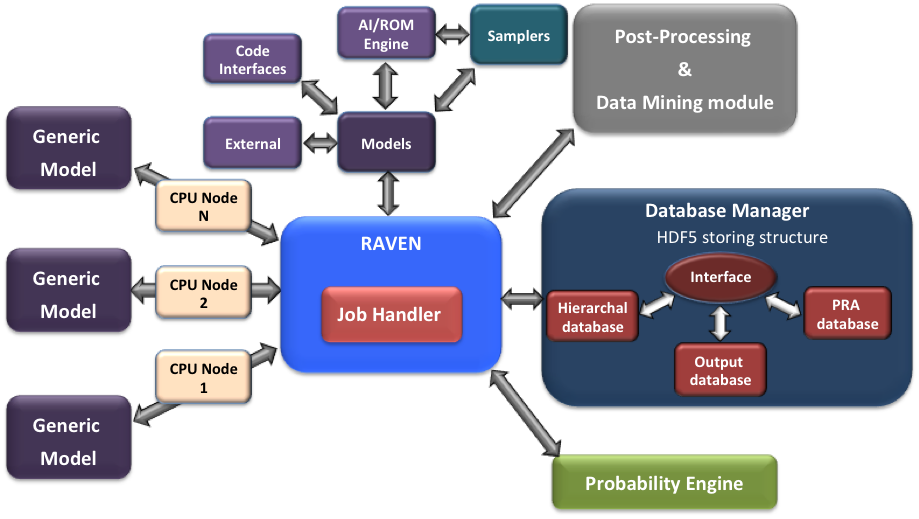
\includegraphics[width=1.0\textwidth]  {pics/RavenFramework.png}
  \caption{RAVEN framework layout}
  \label{fig:RAVENframeworkLayout}
\end{figure}

Hence, RAVEN is coded in $Python$ and is characterized by an object-oriented design. The core of the analysis performable through RAVEN is represented by a set of basic components (objects) the user can combine, in order to create a custom analysis flow. A list of these components and a summary of their most important functionalities are reported as follows:
\begin{itemize}
\item	Distribution: In order to explore the input/output space, RAVEN requires the capability to perturb the input space (initial conditions and/or model coefficients of a system code). The input space is generally characterized by probability distribution functions (PDFs), which might need to be considered when a perturbation is applied. In this respect, a large library of PDFs is available.
\item Sampler: A proper approach to sample the input space is fundamental for the optimization of the computational time. In RAVEN, a ``sampler'' employs a unique perturbation strategy that is applied to the input space of a system. The input space is defined through the connection of uncertain variables and their relative probability distributions.
\item Model: A model is the representation of a physical system (e.g. Nuclear Power Plant); it is therefore capable of predicting the evolution of a system given a coordinate set in the input space. In addition it can represent an
action on a data in order to extract key features (e.g. Data mining).
\item Reduced Order Model (ROM): The evaluation of the system response, as a function of the coordinates in the input space, is very computationally expensive, especially when brute-force approaches (e.g. Monte Carlo methods) are chosen as the sampling strategy. ROMs are used to lower this cost, reducing the number of needed points and prioritizing the area of the input space that needs to be explored. They can be considered as an artificial representation of the link between the input and output spaces for a particular system.
\end{itemize}
The list above is not comprehensive of all the RAVEN framework components (visualization and storage infrastructure).
\\ Figure~\ref{fig:RAVENframeworkLayout} shows a schematic representation of the whole framework, highlighting the communication pipes among the different modules and engines. As can be seen, in the figure all the components reported above are schematically shown. In addition the data management, mining and processing modules are shown.

\subsubsection{Distribution}
As already mentioned, the perturbation of the input space, through the initial conditions (parameters) affected by uncertainties, needs to be performed by the proper distribution functions. RAVEN provides, through an interface to the BOOST library, the following variate (truncated and not) distributions: Bernoulli, Binomial, Exponential, Logistic, Lognormal, Normal, Poisson, Triangular, Uniform, Weibull, Gamma, and Beta.
\\The usage of uni-variate distributions for sampling initial conditions is based on the assumption that the uncertain parameters are not correlated with each other. Quite often uncertain parameters are subject to correlations and thus the uni-variate approach is not applicable. This happens when a generic outcome is dependent on different phenomena simultaneously (i.e. the outcome dependency description can not be collapsed to a function of a single variable). RAVEN currently supports both N-dimensional (N-D) PDFs. The user can provide the distribution values on either Cartesian or sparse grid, which determines the interpolation algorithm used in the evaluation of the imported CDF/PDF:
\begin{enumerate}
\item N-Dimensional Spline, for Cartesian grids
\item Inverse weight, for sparse grids
\end{enumerate}
Internally, RAVEN provides the needed N-D differentiation and integration algorithms to compute the PDF from the CDF and vice-versa.
\\As already mentioned, the sampling methods use the distributions in order to perform probability-weighted perturbations. For example, in the Monte Carlo approach, a random number $\in [0,1]$ is generated (probability threshold) and the CDF, corresponding to that probability, is inverted in order to retrieve the parameter value usable in the simulation. The existence of the inverse for variate distributions is guaranteed by the monotonicity of the CDF. For N-D distributions this condition is not sufficient since the $CDF(X)\longrightarrow [0,1],X \in  R^{N} $ and therefore it could not be a bijective function. From an application point of view, this means the inverse of a N-D CDF is not unique.
\\As an example, the Figure~\ref{fig:NDDistributionExample} shows a multivariate normal distribution for a pipe failure as function of the pressure and temperature. The plane identifies an isoprobability surface (in this case, a line) that represents a probability threshold of 50 \% in this example.  Hence, the inverse of this CDF is an infinite number of points.
 \\As easily inferable, the standard sampling approach cannot directly be employed. When multivariate distributions are used, RAVEN implements a surface search algorithm for identifying the iso-probability surface location. Once the location of the surface has been found, RAVEN chooses, randomly, one point on it.

\begin{figure}
  \centering
  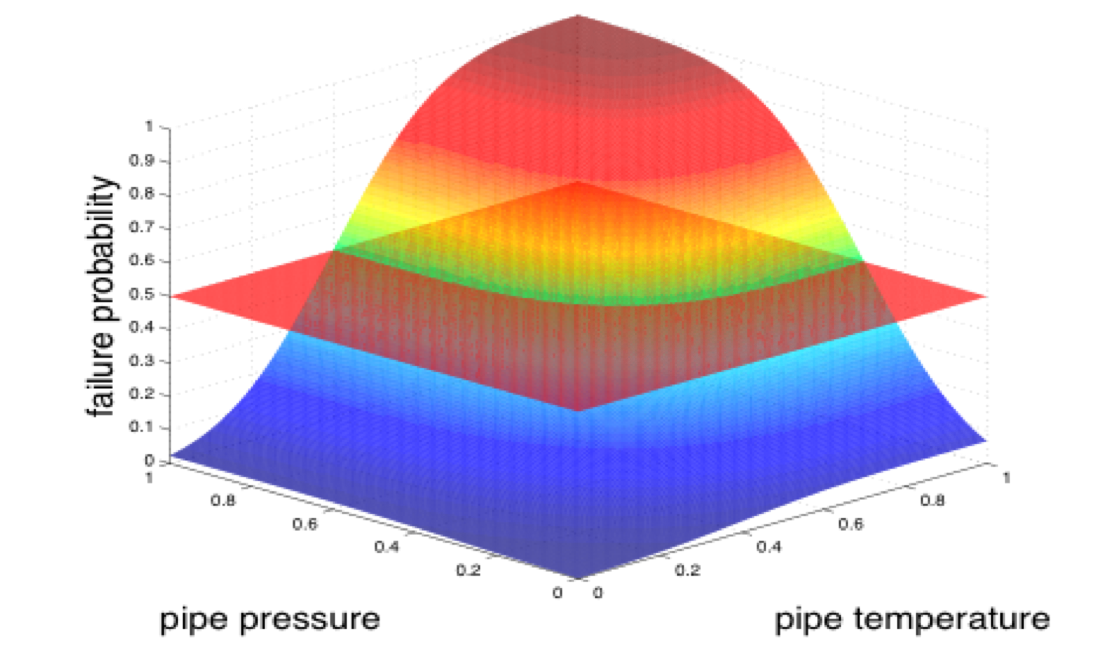
\includegraphics[width=0.5\textwidth]  {pics/NDimensionalDistributionExample.png}
  \caption{2-D CDF, function of pressure and temperature}
  \label{fig:NDDistributionExample}
\end{figure}

\subsubsection{Sampler}

The sampler is probably the most important entity in the RAVEN framework. Indeed, it performs the driving of the specific sampling strategy and, hence, determines the effectiveness of the analysis, from both an accuracy and computational point of view.  The samplers, that are available in RAVEN, can be categorized in three main classes:
\begin{itemize}
 \item Forward
 \item Dynamic Event Tree (DET)
 \item Adaptive
\end{itemize}
\paragraph{Forward Samplers} ~\\
The Forward sampler category collects all the strategies that perform the sampling of the input space without exploiting, through dynamic learning approaches, the information made available from the outcomes of calculation previously performed (adaptive sampling) and the common system evolution (patterns) that different sampled calculations can generate in the phase space (dynamic event tree).
In the RAVEN framework, several different and well-known forward samplers are available:
\begin{itemize}
\item Monte Carlo (MC)
\item Stratified based, whose most known specialization is the Latin Hyper-Cube Sampling (LHS)
\item Grid Based
\item Response Surface Design of Experiment
\item Sparse Grid
\item Factorials
\item Etc.
\end{itemize}
As already mentioned, all these sampling strategies are well known, as well as their properties. Therefore, a detailed investigation of their application is not provided.
%%%%%%%%%%%%%%%%%%%%%%%%%%%%%%%%%%%%%%%%%%%%%%%%%%%%%%%%%%%%%%%%%%%%%%%%%%%%%%%%
\paragraph{Dynamic Event Tree Samplers}~\\
In order to clarify the idea behind the Dynamic Event Tree Sampler currently available in RAVEN, a small overview is needed.
\\In technological complex systems, as nuclear power plants, an accident scenario begins with an initiating event and then evolves over time through the interaction of dynamics and stochastic events. This mutual action leads to the production of infinitely many different scenarios, which define a continuous dynamic event tree with infinite branches. At each time point, the stochastic variability of the accident outcomes is determined by a multivariate probability distribution. The PRA analysis needs an approximation to this distribution for selected consequence variables. A way to achieve this goal is an Event Tree approach. In dynamic PRA analysis, Conventional Event Tree sequences are run simultaneously starting from a single initiating event. The branches occur at user specified times and/or when an action is required by the operator and/or the system, creating a deterministic sequence of events based on the time of their occurrence. One of the disadvantages of this method is that the timing/sequencing of events and system dynamics is not explicitly accounted for in the analysis. In order to overcome these limitations a “dynamic” approach is needed. The Dynamic Event Tree (DET) technique brings several advantages, among which is the fact that it simulates probabilistic system evolution in a way that is consistent with the severe accident model. This leads to a more realistic and mechanistically consistent analysis of the system taken into consideration. The dynamic PRA, in general, and the Dynamic Event Tree methodologies in particular, are designed to take the timing of events explicitly into account, which can become very important especially when uncertainties in complex phenomena are considered. Hence, the main idea of this methodology is to let a system code determine the pathway of an accident scenario.
\\From an application point of view, a N-D grid is built on the CDF space. A single simulation is spawned and a set of triggers is added to the system code control logic. Every time a trigger gets activated (one of the CDF thresholds in the grid is violated), a new set of simulations (branches) is spawned. Each branch carries its own probability.
\\Figure \ref{fig:DETschemeExample} shows a practical example. In this particular case, it is assumed that the
probability failure of a pipe depends on the fluid pressure magnitude. Three probability thresholds are defined on
the cumulative distribution function. One simulation is spawned (0). As soon as the pressure of the fluid reaches a
value corresponding to a 33\% probability (CDF), a stop signal is sent and the framework starts two new
simulations (branches). The branch in which the system evolved to the newer condition (pipe failed, red line)
carries 33\% of the probability, while the other the complementary amount. The same procedure is repeated at
point 2.
\\Generally, not all the input space can be explored using a DET approach. For instance, usually the parameters affected by aleatory uncertainty are sampled using a dynamic event tree approach, while the ones characterized by epistemic uncertainty are sampled through ``forward'' sampling strategies.
\\As already mentioned, this strategy requires a tight interaction between the system code and the sampling driver (i.e., RAVEN framework). In addition, the system code must have a control logic capability (i.e. trigger system). For these reasons, the application of this sampling approach to a generic code needs a larger effort when compared to the other Samplers available in RAVEN. Currently, the DET is fully available for the thermal-hydraulic codes RELAP-7 and RELAP5-3D.
\\In the RAVEN framework, several different DET-based samplers are available:
\begin{itemize}
\item Dynamic Event Tree (aleatory sampling);
\item Hybrid Dynamic Event Tree (aleatory and epistemic sampling);
\item Adaptive Dynamic Event Tree (goal-oriented sampling for aleatory sampling);
\item Adaptive Hybrid Dynamic Event Tree (goal-oriented sampling for aleatory and epistemic sampling).
\end{itemize}

\begin{figure}
  \centering
  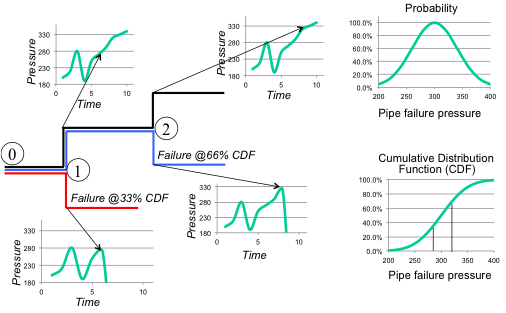
\includegraphics[width=0.7\textwidth]  {pics/DETscheme.png}
  \caption{Dynamic Event Tree simulation pattern}
  \label{fig:DETschemeExample}
\end{figure}

%%%%%%%%%%%%%%%%%%%%%%%%%%%%%%%%%%%%%%%%%%%%%%%%%%%%%%%%%%%%%%%%%%%%%%%%%%%%%%%%
\paragraph{Adaptive Samplers}~\\
A key feature available within RAVEN is the possibility to perform smart sampling (also known as adaptive sampling) as an alternative to classical ``forward'' techniques.
\\The motivation is that nuclear simulations are often computationally expensive, time-consuming, and high dimensional with respect to the number of input parameters. Thus, exploring the space of all possible simulation outcomes is unfeasible using finite computing resources. During simulation-based probabilistic risk analysis, it is important to discover the relationship between a potentially large number of input parameters and the output of a simulation using as few simulation trials as possible.
\\This is a typical context for performing adaptive sampling where a few observations are obtained from the simulation, a reduced order model (ROM) is built to represent the simulation space, and new samples are selected based on the model constructed. The ROM is then updated based on the simulation results of the sampled points. In this way, it is attempted to gain the most information possible with a small number of carefully selected sampled points, limiting the number of expensive trials needed to understand features of the system space.
\\In the RAVEN framework, several different adaptive samplers are available:
\begin{itemize}
\item Limit Surface Search;
\item Adaptive Dynamic Event Tree;
\item Adaptive Hybrid Dynamic Event Tree ;
\item Adaptive Sparse Grid;
\item Adaptive Sobol Decomposition.
\end{itemize}

\subsubsection{Models}
The Model entity, in the RAVEN environment, represents a ``connection pipeline'' between the input and the output space. The RAVEN framework does not own any physical model (i.e. it does not posses the equations needed to simulate a generic physical system, such as Navier-Stocks equations, Maxwell equations, etc.), but implements Application Program Interfaces (APIs) by which any generic model can be integrated and interrogated. The RAVEN framework provides APIs for four different model categories: Codes, Externals, Post-Processors (PPs) and Reduced Order Models (ROMs). In the following paragraphs, a brief explanation of each of this Model categories is reported.
\paragraph{Code} ~\\
The \textit{Code} model represents the communication pipe between the RAVEN framework and any system and physical code. The communication between RAVEN and any driven code is performed through the implementation of interfaces directly operated by the framework.
\\The procedure of coupling a new code/application with RAVEN is a straightforward process. The coupling is performed through a \textit{Python}  interface that interprets the information coming from RAVEN and translates them to the input of the driven code. The coupling procedure does not require modifying RAVEN itself. Instead, the developer creates a new \textit{Python} interface that is going to be embedded in RAVEN at run-time (no need to introduce hard-coded coupling statements).  This interface needs to be placed in a folder (whatever name) located in (see figure~\ref{fig:CodeInterfaceLocation}):
\begin{lstlisting}[language=bash]
 path/to/raven/distribution/raven/framework/CodeInterfaces/
\end{lstlisting}

\begin{figure}
  \centering
  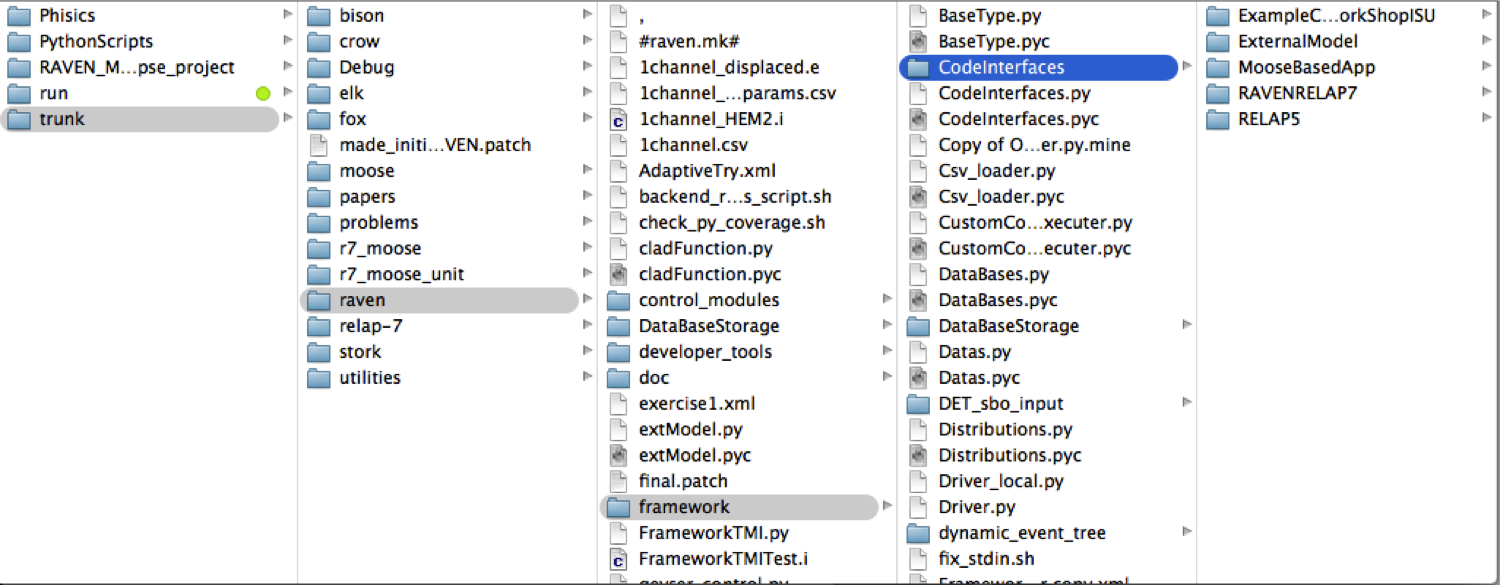
\includegraphics[width=0.8\textwidth]  {pics/CodeInterfaceLocation.png}
  \caption{Code Interface Location}
  \label{fig:CodeInterfaceLocation}
\end{figure}
At the initialization stage, RAVEN imports all the Interfaces that are contained in this directory and performs some preliminary cross-checks.
\\ If the coupled code is parallelized and/or multi-threaded, RAVEN is going to manage the system in order to optimize the computational resources in both workstations and High Performance Computing systems.
\\Currently, RAVEN has APIs for RELAP5-3D, RELAP-7, any MOOSE-based application, SASS and Modelica.
\paragraph{External Model} ~\\
The External model allows the user to create, in a \textit{Python} file (imported, at run-time, in the RAVEN framework), its own model (e.g. set of equations representing a physical model, connection to another code, control logic, etc.). This model will be interpreted/used by the framework and, at run-time, will become part of RAVEN itself.
\paragraph{Post-Processor} ~\\
The Post-Processor model represents the container of all the post-processing capabilities in the RAVEN code. This model is aimed to process the data (for example, derived from the sampling of a physical code) in order to identify representative Figure of Merits. This system has  been designed and, presently, is under heavy development by the whole RAVEN team.  Currently, the following post-processors are available:
\begin{itemize}
 \item \textit{Basic Statistics}, container of the algorithms to compute many of the most important statistical quantities. This post-processor is able to compute mean, sigma/variance, variation coefficient, skewness, kurtosis, median, percentiles and all the principal matrix quantities such as covariance, sensitivity (either leas-squared and variance weighted) and correlation matrices;
 \item \textit{Comparison Statistics}, aimed to employ validation and verification metrics;
 \item \textit{Limit Surface}, aimed to compute the limit surface in the input space (i.e. the hyper-surface that represents the boundary between the failure/success of the system);
 \item \textit{Limit Surface Integral}, intended to compute the integral of the limit surface that corresponds to the probability of failure;
  \item \textit{Safest Point}, provides the coordinates of the farthest point from the limit surface that is given as an input. The safest point coordinates are expected values of the coordinates of the farthest points from the limit surface in the space of the ``controllable'' variables based on the probability distributions of the ``non-controllable'' variables. The term ``controllable'' identifies those variables that are under control during the system operation, while the ``non-controllable'' variables are stochastic parameters affecting the system behavior randomly;
 \item \textit{External Post-Processor}, user-defined post-processor;
 \item \textit{Topological Decomposition}, aimed to compute an approximated hierarchical Morse-Smale complex which will add two columns to a data-set, performing a topological decomposition of such data-set;
 \item \textit{Data Mining}, container of all the RAVEN data mining, clustering and dimensionality reduction techniques aimed to identify dominant and common patterns in high-dimensionality data.
\end{itemize}
\paragraph{Reduced Order Model} ~\\
 As briefly mentioned, a ROM is a mathematical representation of a system, used to predict a selected output space of a physical system.
The ``training'' is a process that uses sampling of the physical model to improve the prediction capability (capability to predict the status of the system given a realization of the input space) of the ROM. More specifically, in RAVEN the Reduced Order Model is trained to emulate a high fidelity numerical representation (system codes) of the physical system. Two general characteristics of these models can be generally assumed (even if exceptions are possible):
\begin{enumerate}
   \item The higher the number of realizations in the training sets, the higher is the accuracy of the prediction performed by the reduced order model. This statement is true for most of the cases although some ROMs might be subject to the over-fitting issues. The over-fitting phenomenon is not discussed here, since its occurrence is highly dependent on the algorithm type, (and there is large number of ROM options available in RAVEN). Every time the user chooses a particular reduced order model algorithm to use, he should consult the relative literature;
   \item The smaller the size of the input domain with respect to the variability of the system response, the more likely the surrogate model will be able to represent the system output space.
\end{enumerate}
In most of the cases of interest, the information that is sought is related to defining the failure boundaries of a system with respect to perturbations in the input space. For this reason, in the development of RAVEN, it has been given priority to the introduction of a class of supervised learning algorithms, which are usually referred to as classifiers. A classifier is a reduced order model that is capable of representing the system behavior through a binary response (failure/success).
\\The first class of classifier introduced has been the Support Vector Machines (SVMs) [reference] with several different kernels (polynomial of arbitrary integer order, radial basis function kernel, sigmoid) followed by a nearest-neighbor based classification using a K-D tree search algorithm. Currently, RAVEN supports around 40 different ROM methodologies. All these supervised learning algorithms have been imported via an API from the scikit-learn [reference] library. In addition, the N-Dimensional spline and the inverse weight methods, that are currently available for the interpolation of N-Dimensional PDF/CDF, can also be used as ROMs.
\subsubsection{Simulation Environment}
RAVEN is perceived by the user as a pool of tools and data. Any action in which the tools are applied to the data is considered a calculation ``step'' in the RAVEN environment. Simplistically, a ``step'' can be seen as a \textbf{transfer function} between the input and output space through a Model (e.g. Code, External, ROM or Post-Processor). One of the most important step in the RAVEN framework is called ``multi-run'', that is aimed to handle calculations that involve multiple runs of a driven code (sampling strategies). Firstly, the RAVEN input file associates the variables to a set of PDFs and to a sampling strategy. The ``multi-run'' step is used to perform several runs in a block of a model (e.g. in a MC sampling).
\begin{figure}[ht]
  \centering
  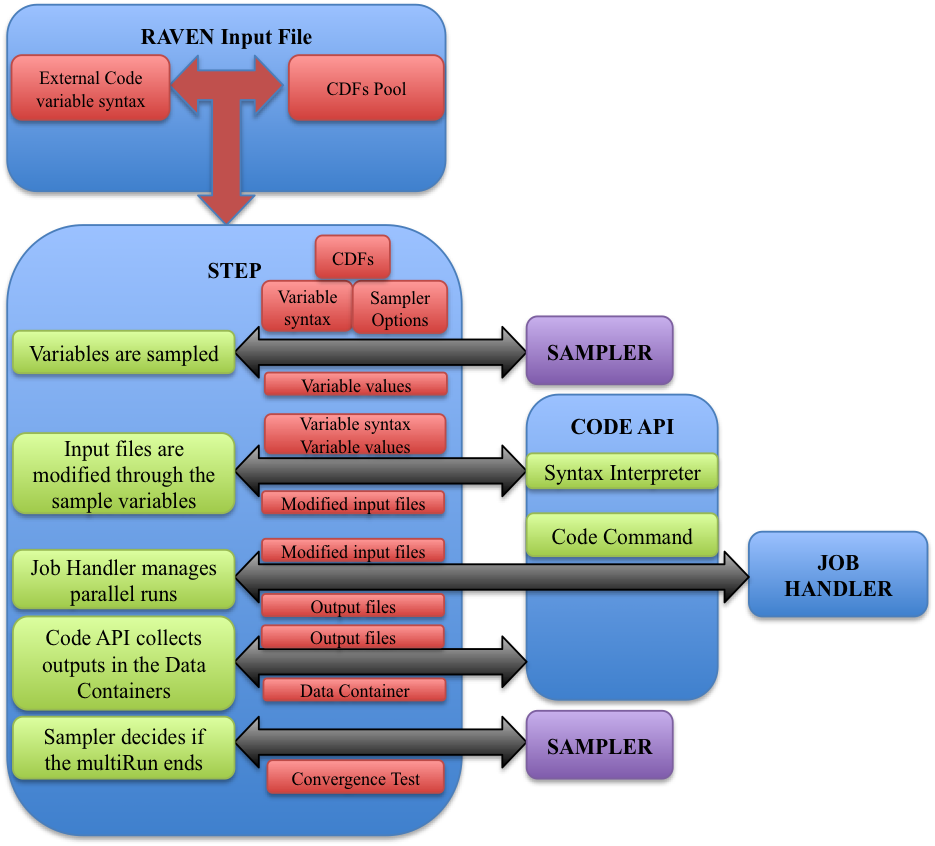
\includegraphics[width=0.8\textwidth]  {pics/MultiRunCalculationFlow.png}
  \caption{Calculation flow for a multi-run sampling}
  \label{fig:multiRun}
\end{figure}
At the beginning of each sub sequential run, the sampler provides the new values of the variables to be perturbed. The code API places those values in the input file. At this point, the code API generates the run command and asks to be queued by the job handler. The job handler manages the parallel execution of as many runs as possible within a user prescribed range and communicates with the step controller when a new set of output files are ready to be processed. The code API receives the new input files and collects the data in the RAVEN internal format. The sampler is queried to assess if the sequence of runs is ended, if not, the step controller asks for a new set of values from the sampler and the sequence is restarted as described in Figure~\ref{fig:multiRun}.
The job handler is currently capable to run different run instances of the code in parallel and can also handle codes that are multi-threaded or using any form of parallel implementation.
RAVEN also has the capability to plot the simulation outcomes while the set of sampling is performed and to store the data for later recovery.

\section{Raven Input Structure}
The RAVEN code does not have a fixed calculation flow, since all of its basic
objects can be combined in order to create a user-defined calculation flow.
%
Thus, its input (XML format) is organized in different XML blocks, each with a
different functionality.
%
The main input blocks are as follows:
\begin{itemize}
  \item \textbf{\textless Simulation\textgreater}: The root node containing the
  entire input, all of
  the following blocks fit inside the \emph{Simulation} block.
  %
  \item \textbf{\textless RunInfo\textgreater}: Specifies the calculation
  settings (number of parallel simulations, etc.).
  %
  \item \textbf{\textless Files\textgreater}: Specifies the files to be
  used in the calculation.
  %
  \item \textbf{\textless Distributions\textgreater}: Defines distributions
  needed for describing parameters, etc.
  %
  \item \textbf{\textless Samplers\textgreater}: Sets up the strategies used for
  exploring an uncertain domain.
  %
  \item \textbf{\textless Functions\textgreater}: Details interfaces to external
  user-defined functions and modules.
  %
  \item \textbf{\textless Models\textgreater}: Specifies codes, ROMs,
  post-processing analysis, etc.
  %
  the user will be building and/or running.
  %
  \item \textbf{\textless Steps\textgreater}: Combines other blocks to detail a
  step in the RAVEN workflow including I/O and computations to be performed.
  %
  \item \textbf{\textless DataObjects\textgreater}: Specifies internal data objects
  used by RAVEN.
  %
  \item \textbf{\textless Databases\textgreater}: Lists the HDF5 databases used
  as input/output to a
  RAVEN run.
  %
  \item \textbf{\textless OutStreamManager\textgreater}: Visualization and
  Printing system block.
  %
\end{itemize}

Each of these blocks are explained in dedicated sections in the following
chapters.
%
\subsection{Comments}
Comments may be included in the RAVEN input using standard XML comments,
using \verb|<!--| and \verb|-->| as shown in the example below.
\begin{lstlisting}[style=XML]
<Simulation>
  ...
  <!-- An Example Comment -->
  <Samplers>
  ...
\end{lstlisting}
Comments may be placed anywhere \emph{except} before the \xmlNode{Simulation}
node or after the \xmlNode{/Simulation} node.
%
Comments outside the root node will cause errors in maintaining input file
compatability.
%
Additionally, comments must completely surround any nodes they comment out.
%
Comments are intended to completely remove blocks of code, or to add readability.
%
For instance, the following is INCORRECT usage:
\begin{lstlisting}[style=XML]
  <!--<Assembler> -->
  <!--</Assembler> -->
\end{lstlisting}
%
and the following is compatible usage for a code block:
%
\begin{lstlisting}[style=XML]
  <!--<Samplers>
    <Monte Carlo name='mc'>
      ...
    </Monte Carlo>
    ...
  </Samplers> -->
\end{lstlisting}


\subsection{Verbosity}
Each block within RAVEN also makes use of a \xmlAttr{verbosity} system,
which allows a user to control the level of output to the user interface.
These settings are declared globally as attributes in the \xmlNode{Simulation} node,
and locally in each block.  The verbosity levels are
\begin{itemize}
\item \xmlString{silent} - Only simulation-breaking errors are displayed.
\item \xmlString{quiet} - Errors as well as warnings are displayed.
\item \xmlString{all} (default) - Errors, warnings, and messages are displayed.
\item \xmlString{debug} - For developers. All errors, warnings, messages, and debug messages are displayed.
\end{itemize}
Examples of verbosity usage are included in many examples throughout this manual.

At the \xmlNode{Simulation} node, global variables can be set, including \xmlAttr{verbosity}.  In addition, the
attribute \xmlAttr{printTimeStamps} can be used to either enable or disable prepending RAVEN output with time stamps
by setting it to \xmlString{true} or \xmlString{false}.


\subsection{External Input Files}
The \xmlNode{ExternalXML} node defines external input file (XML format) that can be used to replace any XML nodes 
under \xmlNode{Simulation} in the RAVEN input file. This node allows a user to load any external input file that contains 
the required XML nodes into the RAVEN input file. Each \xmlNode{ExternalXML} node has the following attributes:
\begin{itemize}
\item \xmlAttr{node}, \xmlDesc{required string attribute}, user-defined XML node of RAVEN input file. 
\item \xmlAttr{xmlToLoad}, \xmlDesc{required string attribute}, file name with its absolute or relative path. Note: if a 
relative path is specified, it must be relative with respect to the RAVEN input file.
\end{itemize}
%
For example, if the file \texttt{Models.xml} contain the required RAVEN input XML node \xmlNode{Models}, 
the RAVEN input file might appear as: 
%
\begin{lstlisting}[style=XML,morekeywords={node,xmlToLoad}]  
<Simulation>
  ...
  <Steps>
    ...
  </Steps>
  ...
  <ExternalXML node='Models' xmlToLoad='external_input/Models.xml'/>
  ...
</Simulation>
\end{lstlisting}
%
Another example, if the file \texttt{MultiRun.xml} contain the required RAVEN input XML node \xmlNode{MultiRun} 
under node \xmlNode{Steps}, the RAVEN input file might appear as:
\begin{lstlisting}[style=XML,morekeywords={node,xmlToLoad}]  
<Simulation>
  ...
  <Steps>
    ...
    <ExternalXML node='MultiRun' xmlToLoad='external_input/MultiRun.xml'/>
    ...
  </Steps>
  ...
</Simulation>
\end{lstlisting}

\section{Manual Formats}
In order to highlight some parts of the manual having a particular meaning (input structure, examples, terminal commands, etc.), specific formats have been used. This section provides the formats with a specific meaning:
\begin{itemize}
\item \textbf{\textit{Python Coding:}}
\begin{lstlisting}[language=python]
class AClass():
  def aMethodImplementation(self):
    pass
\end{lstlisting}
\item \textbf{\textit{XML input example:}}
\begin{lstlisting}[style=XML,morekeywords={anAttribute}]
<MainXMLBlock>
  ...
  <aXMLnode name='anObjectName' anAttribute='aValue'>
     <aSubNode>body</aSubNode>
  </aXMLnode>
  <!-- This is  commented block -->
  ...
</MainXMLBlock>
\end{lstlisting}
\item \textbf{\textit{Bash Commands:}}
\begin{lstlisting}[language=bash]
cd trunk/raven/
./raven_libs_script.sh
cd ../../
\end{lstlisting}
\end{itemize}


\section{Manual Structure}
This manual is intended to provide an overview of the RAVEN capabilities through the explanation of multiple commented examples.
To speed up the learning process, the examples are organized in an ascending complexity order, from simple data manipulation and visualization to
full Probabilistic Risk Assessment and Uncertainty Quantification analysis. In addition, each example is followed by a brief explanation of the theoretical background of the methods that have been used.
\\ It is important to notice that this document is intended to be consulted in conjunction with the user manual ~\cite{RAVENuserManual}.
\\To generalize the examples to any driven software, a simple \texttt{Python} code (conventionally called \textbf{AnalyticBateman}) has been developed (located at ``\textit{doc/user\textunderscore guide/ravenInputs/physicalCode}''). It solves a system of ordinary differential equations (ODEs), of the form:

\begin{equation}
\begin{dcases}
\frac{\mathrm{d} \mathbf{X}}{\mathrm{d} t} = \mathbf{S}-\mathbf{L} \\
 \mathbf{X}(t=0)= \mathbf{X_{0}}
\end{dcases}
\end{equation}
   where:
  \begin{itemize}
     \item $\mathbf{X_{0}}$, initial conditions
     \item $\mathbf{S}$, source terms
     \item $\mathbf{L}$, loss terms
   \end{itemize}

For example, this  code is able to solve a system of equations as follows:
\begin{equation}
  \begin{dcases}
   \frac{\mathrm{d} x_{1}}{\mathrm{d} t} = \phi (t)\times \sigma_{x_{1}}-\lambda_{x_{1}} \\
   \frac{\mathrm{d} x_{2}}{\mathrm{d} t} = \phi (t)\times \sigma_{x_{2}}-\lambda_{x_{2}}+x_{1}(t)\times\lambda_{x_{1}} \\
    x_{1}(t=0)= x_{1}^{0} \\
    x_{2}(t=0)= 0.0
  \end{dcases}
\end{equation}

The input of the \textbf{AnalyticBateman} code is in XML format.
For example, the following is the reference input for a system of 4 Ordinary Differential Equations (ODEs)
that is going to be used for all the examples reported in this manual.  For some examples, the number of
calculated steps might be adjusted for time of calculation (\xmlNode{timeSteps}); however, the operation is
similar for exemplary purposes.

\xmlExample{framework/user_guide/physicalCode/analyticalbateman/Input.xml}{AnalyticalBateman}
The code outputs the time evolution of the 4 variables ($A,B,C,D$) in a CSV file, producing the following output:
\begin{table}[ht]
\centering
\caption{Reference case sample results.}
\label{referenceResults}
\begin{tabular}{lllll}
\textbf{time} & \textbf{A}     & \textbf{C}     & \textbf{B}    & \textbf{D}     \\
0                  & 1.0                       & 1.0                       & 1.0                     & 1.0           \\
2880000.0   & 0.983434738239 & 0.977851848235 & 1.01011506729 & 1.01013172275 \\
5760000.0   & 0.967143884376 & 0.956202457404 & 1.01936231677 & 1.02036100400   \\
8640000.0   & 0.951122892771 & 0.935040450532 & 1.02777406275 & 1.03067925987 \\
10368000.0 & 0.941637968936 & 0.922572556179 & 1.03243314106 & 1.03690947068 \\
12096000.0 & 0.932247632016 & 0.910273757371 & 1.03680933440 & 1.04316700086 \\
13824000.0 & 0.922950938758 & 0.898141730426 & 1.04090912054 & 1.04945015916 \\
15552000.0 & 0.913746955315 & 0.886174183908 & 1.04473885709 & 1.05575729317 \\
17280000.0 & 0.904634757153 & 0.874368858183 & 1.04830478357 & 1.06208678854 \\
20736000.0 & 0.886682064542 & 0.851235986899 & 1.05466958557 & 1.07480659230  \\
24192000.0 & 0.869085647400 & 0.828725658721 & 1.06005115510 & 1.08759739100   \\
27648000.0 & 0.851838435355 & 0.806820896763 & 1.06449535534 & 1.10044757060  \\
31104000.0 & 0.834933498348 & 0.785505191756 & 1.06804634347 & 1.11334606143 \\
34560000.0 & 0.818364043850 & 0.764762489077 & 1.07074662835 & 1.12628231792
\end{tabular}
\end{table}

RAVEN is able to directly retrieve CSV files as output; for this reason, the \textit{\textbf{GenericInterface}} (see ~\cite{RAVENuserManual}-Chapter ``Existing Interfaces'') is used to drive the code.

\section{Run a Single Instance of a Code and Load the Outputs}
The simplest exercise that can be performed is to run the driven code (\textbf{AnalyticBateman}  in our example), loading the results of a single run into RAVEN, printing and plotting some variables.
\\ As detailed in the RAVEN user manual (~\cite{RAVENuserManual}-Chapters ``DataObjects''  and ``Databases'') and in Chapter~/ref{sub:EntitiesAndFlow} RAVEN uses two classes of objects to store the data coming from a driven code (outputs):
\begin{itemize}
  \item \textbf{DataObjects}: The DataObjects represent the preferred way to transfer the information coming from a
   Model (the driven code, in this case) to all the other RAVEN systems (e.g. Out-Stream system, Reduced Order Modeling
   component, etc.).
  \item \textbf{Databases}.
\end{itemize}

As esaly inferable from the user manual (~\cite{RAVENuserManual}-Chapter ``OutStream''), the DataObjects can be exported into a CSV file and plotted (2-D and 3-D plots) linking them into the OutStream system.
\\ The following subsections report examples on how to use these systems running a single instance of the driven code.
\subsection{Single Run using the OutStream system for printing and create basic plots}
\label{sub:SingleRunBasicPlots}
 In this Section, the user can learn how to use RAVEN to run a single instance of a driven code, plotting and printing the
 results.
 \\ The goal of this Section is to learn how to:
 \begin{enumerate}
   \item Set up a simple RAVEN input for running a driven code;
   \item Load the output of the code into the RAVEN DataObjects system;
   \item Print out what contained in the DataObjects;
   \item Generate basic plots of the code results.
\end{enumerate}
In order to accomplish these tasks, the following RAVEN \textbf{Entities} (XML blocks in the input files) are needed:
 \begin{enumerate}
   \item \textbf{\textit{RunInfo}}:
\begin{lstlisting}[style=XML,morekeywords={arg,extension,pauseAtEnd,overwrite}]
    <RunInfo>
      <Sequence>Single, write-History</Sequence>
      <WorkingDir>SectionVI.I</WorkingDir>
      <batchSize>1</batchSize>
    </RunInfo>
\end{lstlisting}
   As reported in Section~\ref{sub:EntitiesAndFlow}, the \textit{RunInfo} \textbf{Entity} is intended to set up the analysis
   that the user wants to perform. In this specific case, two steps (\xmlNode{Sequence}) are going to be sequentially run
   using a single processor (\xmlNode{batchSize}).

   \item \textbf{\textit{Files}}:
\begin{lstlisting}[style=XML,morekeywords={arg,extension,pauseAtEnd,overwrite}]
  <Files>
    <Input name="referenceInput.xml" type="input">referenceInput.xml</Input>
  </Files>
\end{lstlisting}
   Since the driven code uses a single input file, in this Section the original input is placed. As described in the user manual~\cite{}
   the attribute  \xmlAttr{name} represents the alias that is going to be used in all the other input blocks in order to
   refer to this file.
   \item \textbf{\textit{Models}}:
\begin{lstlisting}[style=XML,morekeywords={arg,extension,pauseAtEnd,overwrite}]
   <Models>
      <Code name="testModel" subType="GenericCode">
        <executable>
      ../physicalCode/analyticalbateman/AnalyticalDplMain.py
        </executable>
        <clargs arg="python" type="prepend"/>
        <clargs arg="" extension=".xml" type="input"/>
        <clargs arg="" extension=".csv" type="output"/>
        <prepend>python</prepend>
      </Code>
    <Models>
\end{lstlisting}
  Since the driven code already dumps its outputs in CSV format, there is no need to create
  an ad-hoc code interface and the GenericCode interface can be directly used. In additiom, since the \textbf{AnalyticBateman} code
  is written in \texttt{Python}, it is necessary to specify that the code needs to be run pre-pending the expression ``\texttt{Python}''.
   \item \textbf{\textit{DataObjects}}:
\begin{lstlisting}[style=XML,morekeywords={arg,extension,pauseAtEnd,overwrite}]
  <DataObjects>
    <PointSet name="pointValues">
      <Input>InputPlaceHolder</Input>
      <Output>A,B,C,D</Output>
    </PointSet>
    <HistorySet name="history">
        <Input>InputPlaceHolder</Input>
        <Output>A,B,C,D,time</Output>
    </HistorySet>
  </DataObjects>
\end{lstlisting}
  Int this block, two \textit{DataObjects} are defined: 1) PointSet named ``pointValues'', 2) HistorySet named ``history''.
  Note that a special keyword is inputted in the \xmlNode{Input} node. This keyword is used when a \textit{DataObjects}  \textbf{Entity} needs to be constructed without any linking with respect to the input space. Indeed, in
  this case, the model input space is not perturbed though a sampling strategies; the code is executed through the original
   input file   (``referenceInput.xml''). In the \xmlNode{Output} node all the requested variables are inputted.
   \item \textbf{\textit{OutStreamManager}}:
\begin{lstlisting}[style=XML,morekeywords={arg,extension,pauseAtEnd,overwrite}]
  <OutStreamManager>
    <Print name="pointValues">
      <type>csv</type>
      <source>pointValues</source>
    </Print>
    <Print name="history">
        <type>csv</type>
        <source>history</source>
    </Print>
    <Plot dim="2" name="historyPlot" overwrite="false" verbosity="debug">
        <plotSettings>
            <plot>
                <type>line</type>
                <x>history|Output|time</x>
                <y>history|Output|A</y>
                <color>blue</color>
            </plot>
            <plot>
                <type>line</type>
                <x>history|Output|time</x>
                <y>history|Output|B</y>
                <color>red</color>
            </plot>
            <plot>
                <type>line</type>
                <x>history|Output|time</x>
                <y>history|Output|C</y>
                <color>yellow</color>
            </plot>
            <plot>
                <type>line</type>
                <x>history|Output|time</x>
                <y>history|Output|D</y>
                <color>black</color>
            </plot>
            <xlabel>time (s)</xlabel>
            <ylabel>evolution (kg)</ylabel>
        </plotSettings>
        <actions>
            <how>png,screen</how>
            <title>
                <text> </text>
            </title>
        </actions>
    </Plot>
  </OutStreamManager>
\end{lstlisting}
  In this block, both the Out-Stream types are constructed:
  \begin{itemize}
    \item \textit{Print}:
     \begin{itemize}
       \item named ``pointValues'' connected with the \textit{DataObjects} \textbf{Entity} ``pointValues''
                (\xmlNode{source})
       \item named ``history'' connected with the \textit{DataObjects} \textbf{Entity} ``history'' (\xmlNode{source})
     \end{itemize}
      When this objects get used, all the information contained in the linked  \textit{DataObjects} are going
    to be dumped in CSV files (\xmlNode{type}).
    \item \textit{Plot}: a single \xmlNode{Plot} \textbf{Entity} is defined, containing the line plots of the 4 output variables
    ($A,B,C,D$) in the same figure. This object is going to generate a PNG file and an interactive Plot on
    the screen.
  \end{itemize}
   \item \textbf{\textit{Steps}}:
\begin{lstlisting}[style=XML,morekeywords={arg,extension,pauseAtEnd,overwrite}]
  <Steps>
    <SingleRun name="Single">
      <Input   class="Files"                        type="input">referenceInput.xml</Input>
      <Model  class="Models"                    type="Code">testModel</Model>
      <Output class="DataObjects"            type="PointSet">pointValues</Output>
      <Output class="DataObjects"            type="HistorySet">history</Output>
      <Output class="OutStreamManager" type="Print">pointValues</Output>
    </SingleRun>
    <IOStep name="writeHistory" pauseAtEnd="True">
        <Input    class="DataObjects"            type="HistorySet">history</Input>
        <Output class="OutStreamManager" type="Print">history</Output>
        <Output class="OutStreamManager" type="Plot">historyPlot</Output>
    </IOStep>
  </Steps>
\end{lstlisting}
 %%%%%%%%%%%%%%%%%%%%%%%%%%%%%%%%%%%%%%%%%%%%%%%%%%%%%%%%%%
 %figure history
 \begin{figure}[h!]
  \centering
  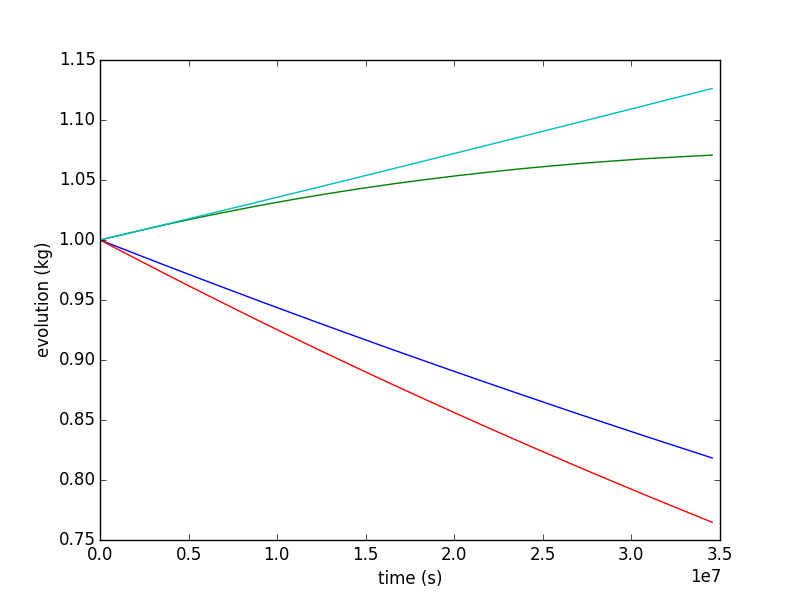
\includegraphics[scale=0.7]{pics/1-historyPlot_line-line-line-line.png}
  \caption{Plot of the history for variables $A,B,C,D$.}
  \label{fig:historyPlotLine}
 \end{figure}
 %%%%%%%%%%%%%%%%%%%%%%%%%%%%%%%%%%%%%%%%%%%%%%%%%%%%%%%%%%
   Finally, all the previously defined \textbf{Entities} can be combined in the \xmlNode{Steps} block. Thus,
   two \xmlNode{Steps} have been inputted:
   \begin{itemize}
     \item \xmlNode{SingleRun} named ``Single'', used to run the single instance of the driven code and collect
     the outputs in the two \textit{DataObjects}. In addition, it can be seen that an additional object has been
     placed among the \xmlNode{Output}(s). Indeed, an  \textit{OutStreamManager} can be an \xmlNode{Output} in
     any Step type (as long as the linked \textit{DataObjects} plays a whatever role in the Step)
     \item  \xmlNode{IOStep} named ``writeHistory'', used to 1) dump the ``history'' \textit{DataObjects}
     \textbf{Entity} in a CSV file and 2) plot the data in the PNG file and on the screen.
   \end{itemize}
\end{enumerate}
 Tables~\ref{historyVI.I} and \ref{pointValuesVI.I} show the results dumped by the OutStreams \textit{Print}.
 As previously mentioned, Figure~\ref{fig:historyPlotLine} reports the four plots (four variables) drawn in the same picture.
 % table history set
\begin{table}[h!]
\centering
\caption{``history'' HistorySet CSV output file.}
\label{historyVI.I}
\begin{tabular}{|c|c|c|c|c|}
\hline
\textbf{A}                        & \textbf{C}                       & \textbf{B}                       & \textbf{D}                       & \textbf{time}                 \\ \hline
1                                 & 1                                & 1                                & 1                                & 0                             \\ \hline
0.983434738                       & 0.977851848                      & 1.010115067                      & 1.010131723                      & 2880000                       \\ \hline
0.967143884                       & 0.956202457                      & 1.019362317                      & 1.020361004                      & 5760000                       \\ \hline
0.951122893                       & 0.935040451                      & 1.027774063                      & 1.03067926                       & 8640000                       \\ \hline
0.941637969                       & 0.922572556                      & 1.032433141                      & 1.036909471                      & 10368000                      \\ \hline
0.932247632                       & 0.910273757                      & 1.036809334                      & 1.043167001                      & 12096000                      \\ \hline
0.922950939                       & 0.89814173                       & 1.040909121                      & 1.049450159                      & 13824000                      \\ \hline
0.913746955                       & 0.886174184                      & 1.044738857                      & 1.055757293                      & 15552000                      \\ \hline
0.904634757                       & 0.874368858                      & 1.048304784                      & 1.062086789                      & 17280000                      \\ \hline
0.886682065                       & 0.851235987                      & 1.054669586                      & 1.074806592                      & 20736000                      \\ \hline
0.869085647                       & 0.828725659                      & 1.060051155                      & 1.087597391                      & 24192000                      \\ \hline
\multicolumn{1}{|l|}{0.851838435} & \multicolumn{1}{l|}{0.806820897} & \multicolumn{1}{l|}{1.064495355} & \multicolumn{1}{l|}{1.100447571} & \multicolumn{1}{l|}{27648000} \\ \hline
\multicolumn{1}{|l|}{0.834933498} & \multicolumn{1}{l|}{0.785505192} & \multicolumn{1}{l|}{1.068046343} & \multicolumn{1}{l|}{1.113346061} & \multicolumn{1}{l|}{31104000} \\ \hline
\multicolumn{1}{|l|}{0.818364044} & \multicolumn{1}{l|}{0.764762489} & \multicolumn{1}{l|}{1.070746628} & \multicolumn{1}{l|}{1.126282318} & \multicolumn{1}{l|}{34560000} \\ \hline
\end{tabular}
\end{table}
% table point set
\begin{table}[h!]
\centering
\caption{``pointValues'' PointSet CSV output file.}
\label{pointValuesVI.I}
\begin{tabular}{|c|c|c|c|c|}
\hline
\textbf{InputPlaceHolder} & \textbf{A}    & \textbf{C}     & \textbf{B}    & \textbf{D}    \\ \hline
0.0                       & 0.81836404385 & 0.764762489077 & 1.07074662835 & 1.12628231792 \\ \hline
\end{tabular}
\end{table}


\subsection{Single Run using the OutStream System to Sub-plot and Selectively print.}
This Section shows how to use RAVEN to create sub-plots (multiple plots in the same figure) and
how to select only some variable from the \textit{DataObjects} in the \textit{Print} OutStream.
 \\ The goals of this Section are about learning how to:
 \begin{enumerate}
   \item Print out what contained in the DataObjects, selecting only few variables
   \item Generate sub-plots (multiple plots in the same figure) of the code results
\end{enumerate}

To accomplish these tasks, the \textit{OutStreamManager} \textbf{Entity} in the input defined in the previous Section (~\ref{sub:SingleRunBasicPlots}) needs to be modified as follows:
\begin{enumerate}
   \item \textbf{\textit{Print}}:
   \begin{lstlisting}[style=XML,morekeywords={arg,extension,pauseAtEnd,overwrite}]
    <Print name="pointValues">
      <type>csv</type>
      <source>pointValues</source>
      <what>Output</what>
    </Print>
    <Print name="history">
        <type>csv</type>
        <source>history</source>
        <what>Output|A,Output|D</what>
    </Print>
   \end{lstlisting}
   With respect to the \textit{Print} nodes defined in the previous Section (~\ref{sub:SingleRunBasicPlots}), it can
   be noticed that an additional node has been added: \xmlNode{what}. The \textit{Print} \textbf{Entity}
   ``pointValues'' is going to extract and dump only the variables that are part of the Output space
   ($A,B,C,D$ and not $InputPlaceHolder$).  The \textit{Print} \textbf{Entity} ``history'' is instead going to print
   the Output space variables $A$ and $D$.

   \item \textbf{\textit{Plot}}:
   \begin{lstlisting}[style=XML,morekeywords={arg,extension,pauseAtEnd,overwrite}]
    <Plot dim="2" name="historyPlot" overwrite="false" verbosity="debug">
        <plotSettings>
            <gridSpace>2 2</gridSpace>
            <plot>
                <type>line</type>
                <x>history|Output|time</x>
                <y>history|Output|A</y>
                <color>blue</color>
                <gridLocation>
                  <x>0</x>
                  <y>0</y>
                </gridLocation>
            </plot>
            <plot>
                <type>line</type>
                <x>history|Output|time</x>
                <y>history|Output|B</y>
                <color>red</color>
                <gridLocation>
                    <x>1</x>
                    <y>0</y>
                </gridLocation>
            </plot>
            <plot>
                <type>line</type>
                <x>history|Output|time</x>
                <y>history|Output|C</y>
                <color>yellow</color>
                <gridLocation>
                    <x>0</x>
                    <y>1</y>
                </gridLocation>
            </plot>
            <plot>
                <type>line</type>
                <x>history|Output|time</x>
                <y>history|Output|D</y>
                <color>black</color>
                <gridLocation>
                    <x>1</x>
                    <y>1</y>
                </gridLocation>
            </plot>
            <xlabel>time (s)</xlabel>
            <ylabel>evolution (kg)</ylabel>
        </plotSettings>
        <actions>
            <how>png,screen</how>
            <title>
                <text> </text>
            </title>
        </actions>
    </Plot>
\end{lstlisting}
 Note that the  \textit{Plot} \textbf{Entity} does not differ much with respect to the one in
 Section~\ref{sub:SingleRunBasicPlots}: 1) the additional sub-node \xmlNode{gridSpace}  has been added.
 This node is needed to define how the figure needs to be partitioned (discretization of the grid). In this case
 a 2 by 2 grid is requested. 2) in each \xmlNode{plot} the node \xmlNode{gridLocation} is placed in
 order to specify in which position the relative plot needs to be placed. For example, in the following grid
 location, the relative plot is going to be placed at the bottom-right corner.
  \begin{lstlisting}[style=XML,morekeywords={arg,extension,pauseAtEnd,overwrite}]
   <gridLocation>
      <x>1</x>
      <y>1</y>
   </gridLocation>
   \end{lstlisting}
 \end{enumerate}
The CSV tables generated by the \textit{Print} \textbf{Entities} are not reported, since the only differences with respect to Tables ~\ref{historyVI.I} and ~\ref{pointValuesVI.I} are related to the number of columns (variables)
dumped out.
\\Figure~\ref{fig:historySubPlotLine} reports the four plots (four variables) drawn in the same picture.
 %figure history sublots
 \begin{figure}[h!]
  \centering
  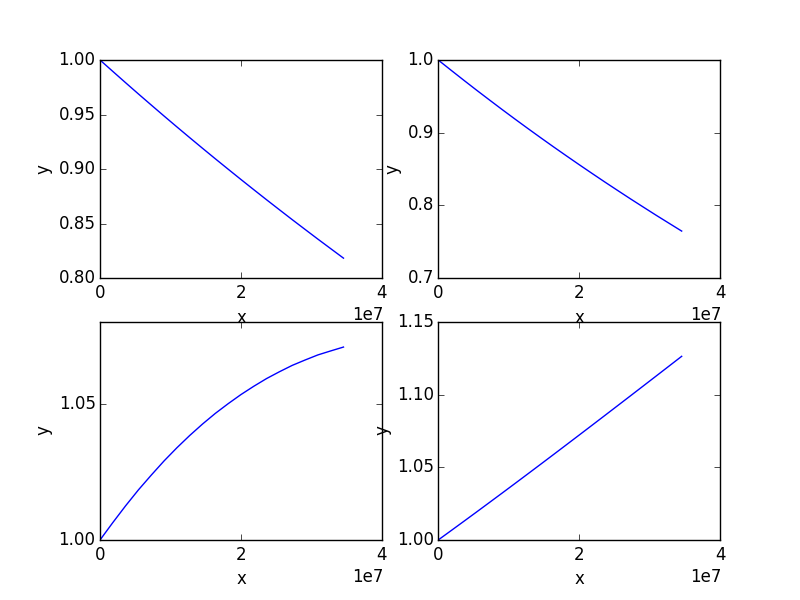
\includegraphics[scale=0.7]{pics/1-historyPlot_line-line-line-line-subPlots.png}
  \caption{Subplot of the history for variables $A,B,C,D$.}
  \label{fig:historySubPlotLine}
 \end{figure}


\begin{appendices}
 \section{Running RAVEN}

% I don't think this is mentioned earlier? Andrea answers :D It mentioned in the Introduction
%As already mentioned, 
The RAVEN code is a mixture of C++, C, and Python software. The entry point 
resides on the Python side and is accessible via a command line interface.
%
After following the instructions in the previous Section, RAVEN is ready to be
used. 
%
The RAVEN driver is contained in the folder ``\texttt{raven/framework}.''
%
To run RAVEN, open a terminal and use the following command (replace \texttt{<inputFileName.xml>} with your RAVEN input file):

\begin{lstlisting}[language=bash]
python raven/framework/Driver.py <inputFileName.xml>
\end{lstlisting}

\end{appendices}
%\appendix
\section{Appendix: Example Primer}
\label{sec:examplePrimer}
In this Appendix, a set of examples are reported. In order to be as general as possible, the \textit{Model} type ``ExternalModel'' has been used.
%%%% EXAMPLE 1 
\subsection{Example 1.}
\label{subsec:ex1}
This simple example is about the construction of a ``Lorentz attractor'', sampling the relative input space. The parameters that are sampled represent the initial coordinate (x0,y0,z0) of the attractor origin. 

\begin{lstlisting}[style=XML,morekeywords={debug,re,seeding,class,subType,limit}]
<?xml version="1.0" encoding="UTF-8"?>
<Simulation verbosity="debug">
<!-- RUNINFO -->
<RunInfo>
    <WorkingDir>externalModel</WorkingDir>
    <Sequence>FirstMRun</Sequence>
    <batchSize>3</batchSize>
</RunInfo>
<!-- Files -->
<Files>
    <Input name='lorentzAttractor.py' type=''>lorentzAttractor</Input>
</Files>
<!-- STEPS -->
<Steps>
    <MultiRun name='FirstMRun'  re-seeding='25061978'>
        <Input   class='Files'     type=''               >lorentzAttractor.py</Input>
        <Model   class='Models'    type='ExternalModel'  >PythonModule</Model>
        <Sampler class='Samplers'  type='MonteCarlo'     >MC_external</Sampler>
        <Output  class='DataObjects'     type='HistorySet'      >testPrintHistorySet</Output>
        <Output  class='Databases' type='HDF5'           >test_external_db</Output>
        <Output  class='OutStreamManager' type='Print'   >testPrintHistorySet_dump</Output>
    </MultiRun >
</Steps>
<!-- MODELS -->
<Models>
    <ExternalModel name='PythonModule' subType='' ModuleToLoad='externalModel/lorentzAttractor'>  
       <variable>sigma</variable>
       <variable>rho</variable>
       <variable>beta</variable>
       <variable>x</variable>
       <variable>y</variable>
       <variable>z</variable>
       <variable>time</variable>
       <variable>x0</variable>
       <variable>y0</variable>
       <variable>z0</variable>
    </ExternalModel>
</Models>
<!-- DISTRIBUTIONS -->
<Distributions>
    <Normal name='x0_distrib'>
        <mean>4</mean>
        <sigma>1</sigma>
    </Normal>
    <Normal name='y0_distrib'>
        <mean>4</mean>
        <sigma>1</sigma>
    </Normal>
    <Normal name='z0_distrib'>
        <mean>4</mean>
        <sigma>1</sigma>
    </Normal>
</Distributions>
<!-- SAMPLERS -->
<Samplers>
    <MonteCarlo name='MC_external'>
      <sampler_init>
        <limit>3</limit>
      </sampler_init>
      <variable name='x0' >
        <distribution  >x0_distrib</distribution>
      </variable>
      <variable name='y0' >
        <distribution  >y0_distrib</distribution>
      </variable>
      <variable name='z0' >
        <distribution  >z0_distrib</distribution>
      </variable>
    </MonteCarlo>
</Samplers>
<!-- DATABASES -->
<Databases>
  <HDF5 name="test_external_db"/>
</Databases>
<!-- OUTSTREAMS -->
<OutStreamManager>
  <Print name='testPrintHistorySet_dump'>
    <type>csv</type>
    <source>testPrintHistorySet</source>
  </Print>
</OutStreamManager>
<!-- DATA OBJECTS -->
<DataObjects>
    <HistorySet name='testPrintHistorySet'>
        <Input>x0,y0,z0</Input>
        <Output>time,x,y,z</Output>
   </HistorySet>
</DataObjects>
</Simulation>
\end{lstlisting}
The Python \textit{ExternalModel} is reported below:
\begin{lstlisting}[language=python]
import numpy as np

def run(self,Input):
  max_time = 0.03
  t_step = 0.01

  numberTimeSteps = int(max_time/t_step)

  self.x = np.zeros(numberTimeSteps)
  self.y = np.zeros(numberTimeSteps)
  self.z = np.zeros(numberTimeSteps)
  self.time = np.zeros(numberTimeSteps)

  self.x0 = Input['x0']
  self.y0 = Input['y0']
  self.z0 = Input['z0']

  self.x[0] = Input['x0']
  self.y[0] = Input['y0']
  self.z[0] = Input['z0']
  self.time[0]= 0

  for t in range (numberTimeSteps-1):
    self.time[t+1] = self.time[t] + t_step
    self.x[t+1]    = self.x[t] +  self.sigma*
                      (self.y[t]-self.x[t]) * t_step
    self.y[t+1]    = self.y[t] + (self.x[t]*
                      (self.rho-self.z[t])-self.y[t]) * t_step
    self.z[t+1]    = self.z[t] + (self.x[t]*
                          self.y[t]-self.beta*self.z[t]) * t_step
\end{lstlisting}
%%%% EXAMPLE 2 
\subsection{Example 2.}
\label{subsec:ex1}
This example shows a slightly more complicated example, that employs the usage of:
\begin{itemize}
    \item \textit{Samplers:} Grid and Adaptive;
    \item \textit{Models:} External, Reduce Order Models and Post-Processors;
    \item \textit{OutStreams:} Prints and Plots;
    \item \textit{Data Objects:} PointSets;
    \item \textit{Functions:} ExternalFunctions.
\end{itemize}
The goal of this input is to compute the ``SafestPoint''.
It provides the coordinates of the farthest
point from the limit surface that is given as an input.
%
The safest point coordinates are expected values of the coordinates of the
farthest points from the limit surface in the space of the ``controllable''
variables based on the probability distributions of the ``non-controllable''
variables.

The term ``controllable'' identifies those variables that are under control
during the system operation, while the ``non-controllable'' variables are
stochastic parameters affecting the system behaviour randomly.

The ``SafestPoint'' post-processor requires the set of points belonging to the
limit surface, which must be given as an input.

\begin{lstlisting}[style=XML,morekeywords={debug,re,seeding,class,subType,limit}]
<Simulation verbosity='debug'>

<!-- RUNINFO -->
<RunInfo>
  <WorkingDir>SafestPointPP</WorkingDir>
  <Sequence>pth1,pth2,pth3,pth4</Sequence>
  <batchSize>50</batchSize>
</RunInfo>

<!-- STEPS -->
<Steps>  
  <MultiRun name = 'pth1' pauseAtEnd = 'False'>
    <Sampler  class = 'Samplers'  type = 'Grid'           >grd_vl_ql_smp_dpt</Sampler>
    <Input    class = 'DataObjects'     type = 'PointSet'   >grd_vl_ql_smp_dpt_dt</Input>
    <Model    class = 'Models'    type = 'ExternalModel'  >xtr_mdl</Model>
    <Output   class = 'DataObjects'     type = 'PointSet'   >nt_phy_dpt_dt</Output>    
  </MultiRun >
  
  <MultiRun name = 'pth2' pauseAtEnd = 'True'>
    <Sampler          class = 'Samplers'  type = 'Adaptive'      >dpt_smp</Sampler>
    <Input            class = 'DataObjects'     type = 'PointSet'  >bln_smp_dt</Input>   
    <Model            class = 'Models'    type = 'ExternalModel' >xtr_mdl</Model>
    <Output           class = 'DataObjects'     type = 'PointSet'  >nt_phy_dpt_dt</Output>            
    <SolutionExport   class = 'DataObjects'     type = 'PointSet'  >lmt_srf_dt</SolutionExport>
  </MultiRun>
  
  <PostProcess name='pth3' pauseAtEnd = 'False'>
    <Input    class = 'DataObjects'          type = 'PointSet'       >lmt_srf_dt</Input>
    <Model    class = 'Models'         type = 'PostProcessor'  >SP</Model>
    <Output   class = 'DataObjects'          type = 'PointSet'     >sfs_pnt_dt</Output>
  </PostProcess>  
  
  <OutStreamStep name = 'pth4' pauseAtEnd = 'True'>
  	<Input  class = 'DataObjects'            type = 'PointSet'  >lmt_srf_dt</Input>
  	<Output class = 'OutStreamManager' type = 'Print'         >lmt_srf_dmp</Output>
    <Input  class = 'DataObjects'            type = 'PointSet'  >sfs_pnt_dt</Input>
  	<Output class = 'OutStreamManager' type = 'Print'         >sfs_pnt_dmp</Output>
  </OutStreamStep>
</Steps>

<!-- DATA OBJECTS -->
<DataObjects> 
  <PointSet name = 'grd_vl_ql_smp_dpt_dt'>
    <Input>x1,x2,gammay</Input>
    <Output>OutputPlaceHolder</Output>
  </PointSet>
  
  <PointSet name = 'nt_phy_dpt_dt'>
    <Input>x1,x2,gammay</Input>
    <Output>g</Output>
  </PointSet>
    
  <PointSet name = 'bln_smp_dt'>
    <Input>x1,x2,gammay</Input>
    <Output>OutputPlaceHolder</Output>
  </PointSet>
    
  <PointSet name = 'lmt_srf_dt'>
    <Input>x1,x2,gammay</Input>
    <Output>g_zr</Output>
  </PointSet>
  
  <PointSet name = 'sfs_pnt_dt'>
    <Input>x1,x2,gammay</Input>
    <Output>p</Output>
  </PointSet>
</DataObjects>

<!-- DISTRIBUTIONS -->
<Distributions>
  <Normal name = 'x1_dst'>
    <upperBound>10</upperBound>
    <lowerBound>-10</lowerBound>
  	<mean>0.5</mean>
    <sigma>0.1</sigma>
  </Normal>
  
  <Normal name = 'x2_dst'>
    <upperBound>10</upperBound>
    <lowerBound>-10</lowerBound>
    <mean>-0.15</mean>
    <sigma>0.05</sigma>
  </Normal>
  
  <Normal name = 'gammay_dst'>
    <upperBound>20</upperBound>
    <lowerBound>-20</lowerBound>
    <mean>0</mean>
    <sigma>15</sigma>
  </Normal>
</Distributions>

<!-- SAMPLERS -->
<Samplers>  
  <Grid name = 'grd_vl_ql_smp_dpt'>
    <variable name = 'x1' >
      <distribution>x1_dst</distribution>
      <grid type = 'value' construction = 'equal' steps = '10' upperBound = '10'>2</grid>
    </variable>  
    <variable name='x2' >
      <distribution>x2_dst</distribution>
      <grid type = 'value' construction = 'equal' steps = '10' upperBound = '10'>2</grid>
    </variable>
    <variable name='gammay' >
      <distribution>gammay_dst</distribution>
      <grid type = 'value' construction = 'equal' steps = '10' lowerBound = '-20'>4</grid>
    </variable>
  </Grid>
  
  <Adaptive name = 'dpt_smp' verbosity='debug'>
    <ROM              class = 'Models'    type = 'ROM'           >accelerated_ROM</ROM>
    <Function         class = 'Functions' type = 'External'      >g_zr</Function>
    <TargetEvaluation class = 'DataObjects'     type = 'PointSet'  >nt_phy_dpt_dt</TargetEvaluation>
    <Convergence limit = '3000' forceIteration = 'False' weight = 'none' persistence = '5'>1e-2</Convergence>
      <variable name = 'x1'>
        <distribution>x1_dst</distribution>
      </variable>
      <variable name = 'x2'>
        <distribution>x2_dst</distribution>
      </variable>
      <variable name = 'gammay'>
        <distribution>gammay_dst</distribution>
      </variable>
  </Adaptive>
</Samplers>

<!-- MODELS -->
<Models>  
  <ExternalModel name = 'xtr_mdl' subType = '' ModuleToLoad = 'SafestPointPP/safest_point_test_xtr_mdl'>
    <variable>x1</variable>
    <variable>x2</variable>
    <variable>gammay</variable>
    <variable>g</variable>
  </ExternalModel>
  
  <ROM name = 'accelerated_ROM' subType = 'SciKitLearn'>
    <Features>x1,x2,gammay</Features>
    <Target>g_zr</Target>
    <SKLtype>svm|SVC</SKLtype>
    <kernel>rbf</kernel>
    <gamma>10</gamma>
    <tol>1e-5</tol>
    <C>50</C>
  </ROM>

  <PostProcessor name='SP' subType='SafestPoint'>
    <!-- List of Objects (external with respect to this PP) needed by this post-processor -->
    <Distribution     class = 'Distributions'  type = 'Normal'>x1_dst</Distribution>
    <Distribution     class = 'Distributions'  type = 'Normal'>x2_dst</Distribution>
    <Distribution     class = 'Distributions'  type = 'Normal'>gammay_dst</Distribution>
    <!- end of the list -->
    <controllable>
    	<variable name = 'x1'>
    		<distribution>x1_dst</distribution>
    		<grid type = 'value' steps = '20'>1</grid>   		
    	</variable>
    	<variable name = 'x2'>
    		<distribution>x2_dst</distribution>
    		<grid type = 'value' steps = '20'>1</grid>   		
    	</variable>
    </controllable>
    <non-controllable>
    	<variable name = 'gammay'>
    		<distribution>gammay_dst</distribution>
    		<grid type = 'value' steps = '20'>2</grid>
    	</variable> 	
    </non-controllable>
  </PostProcessor>
</Models>

<!-- FUNCTIONS -->
<Functions>
  <External name='g_zr' file='SafestPointPP/safest_point_test_g_zr.py'>
    <variable>g</variable>
  </External>
</Functions>

<!-- OUT-STREAMS -->
<OutStreamManager> 
  <Print name = 'lmt_srf_dmp'>
  	<type>csv</type>
  	<source>lmt_srf_dt</source>
  </Print>
  
  <Print name = 'sfs_pnt_dmp'>
  	<type>csv</type>
  	<source>sfs_pnt_dt</source>
  </Print>
</OutStreamManager>

</Simulation>
\end{lstlisting}
The Python \textit{ExternalModel} is reported below:
\begin{lstlisting}[language=python]
def run(self,Input): 
  self.g = self.x1+4*self.x2-self.gammay
\end{lstlisting}
The ``Goal Function'',the function that defines the transitions with respect the input space coordinates, is as follows:
\begin{lstlisting}[language=python]
def __residuumSign(self):
  if self.g<0 : return  1
  else        : return -1
\end{lstlisting}

%%%%% EXAMPLE 3
%\subsection{Example3}
%\label{subsec:ex1}
%example 3



    % ---------------------------------------------------------------------- %
    % References
    %
    \clearpage
    % If hyperref is included, then \phantomsection is already defined.
    % If not, we need to define it.
    \providecommand*{\phantomsection}{}
    \phantomsection
    \addcontentsline{toc}{section}{References}
    \bibliographystyle{ieeetr}
    \bibliography{raven_user_guide}


    % ---------------------------------------------------------------------- %
    %

    % \printindex

    %\include{distribution}

\end{document}
